\documentclass[a4paper]{article}

\usepackage{listings}
\usepackage{xcolor}
\usepackage{graphics}

\definecolor{codegreen}{rgb}{0,0.6,0}
\definecolor{codegray}{rgb}{0.5,0.5,0.5}
\definecolor{codepurple}{rgb}{0.58,0,0.82}
\definecolor{backcolour}{rgb}{0.95,0.95,0.92}

\lstdefinestyle{mystyle}{
    backgroundcolor=\color{backcolour},   
    commentstyle=\color{codegreen},
    keywordstyle=\color{magenta},
    numberstyle=\tiny\color{codegray},
    stringstyle=\color{codepurple},
    basicstyle=\ttfamily\footnotesize,
    breakatwhitespace=false,         
    breaklines=true,                 
    captionpos=b,                    
    keepspaces=true,                 
    numbers=left,                    
    numbersep=5pt,                  
    showspaces=false,                
    showstringspaces=false,
    showtabs=false,                  
    tabsize=2
}

\lstset{style=mystyle}

\begin{document}

\section{Installing on Linux}
I remember that you are on a Ubuntu distribution,  you can install git on you computer with the following command:
\begin{lstlisting}[language=bash]
\$ sudo apt install git-all
\end{lstlisting}

\section{Cloning a Project from a Remote Repo}

You can copy the PDE project from the remote repository at the below link with the following cml command:
https://github.com/LiuBohi/pde.git

\begin{lstlisting}[language=bash]
\$ git clone <remote-url> <working-directory-name>
\end{lstlisting}

\section{Routine workflow:"Edit/Stage/Commit/Push" Cycle}
You can edit your files as usual, which produces "unstaged" file changes.
Stage file changes, which produces "Staged" file changes.
\begin{lstlisting}[language=bash]
\$ git add <file>  # for new and modified files
\$ git rm <file>   # for deleted files
\$ git mv <old-file-name> <new-file-name>  # for renamed files

\$ git commit -m "<your message>" # commit all staged file changes

\$ git push <remote-name> <local-branch-name>  # Push
\end{lstlisting}

Or you can stage all files with changes
\begin{lstlisting}[language=bash]
\$ git add --all
\$ git commit -m "<your message>"
\$ git push
\end{lstlisting}

\begin{figure}
\centerline{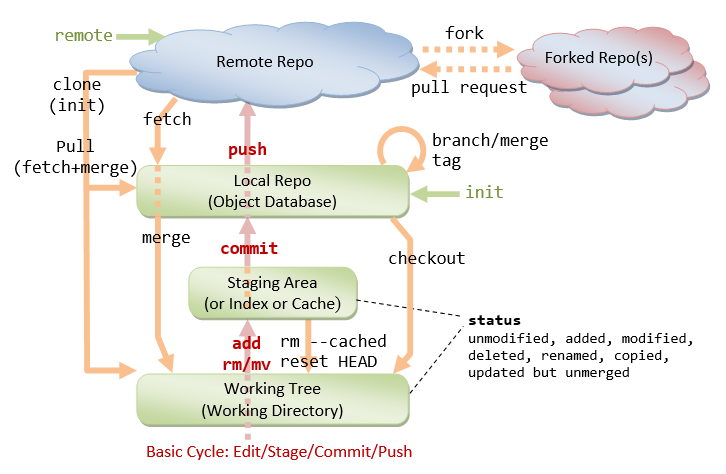
\includegraphics{Git_StorageDataFlow.png}}
\caption{Git Workflow}
\end{figure}

\end{document}

